\documentclass[12pt,twocolumn]{article}

\usepackage[utf8]{inputenc}
\usepackage[T1]{fontenc}
\usepackage[english]{babel}
\usepackage[a4paper,left=0.5cm,right=0.5cm,top=0.5cm,bottom=0.5cm]{geometry}
\usepackage{amsmath, amssymb, amsthm}
\usepackage{graphicx}
\usepackage{hyperref}
\usepackage{csquotes}
\linespread{0.95}
\usepackage{titlesec}
\titlespacing*{\section}{0pt}{*1.0}{*0.4}
\titlespacing*{\subsection}{0pt}{*0.8}{*0.3}
\titlespacing*{\subsubsection}{0pt}{*0.7}{*0.2}
\titlespacing*{\paragraph}
{0pt}    % linker Einzug
{0.5ex}  % Abstand davor
{0.5em}  % Abstand danach
\usepackage{enumitem}
\usepackage{libertinus}

\begin{document}
    \section*{Prüfverfahren (ZP, ZFP) \& Mechanische Eigenschaften}
    \subsection{Zertörende Werkstoffprüfungen}
    \paragraph{Härteprüfung}\mbox{}\\
     \begin{minipage}[t]{0.32\columnwidth}
        Brinell
    \end{minipage}\hfill
    \begin{minipage}[t]{0.32\columnwidth}
        Rockwell
    \end{minipage}\hfill
    \begin{minipage}[t]{0.32\columnwidth}
        Vickers
    \end{minipage}\hfill
    \paragraph{Zugversuch}\mbox{}\\
    \begin{minipage}[t]{0.45\columnwidth}
        \begin{itemize}[label={}, leftmargin=*,  itemsep=0.1em]
            \item Nennspannung: \\ $\sigma = \frac{F}{S_0}\qquad[\sigma]=\frac{N}{m^2}$
            \item Dehnung: \\ $\epsilon = \frac{\Delta l}{l_0}\qquad[\epsilon]=m$
            \item E-Modul: \\ $E = \frac{\sigma}{\epsilon}\qquad[E]=GPa$
        \end{itemize}
    \end{minipage}\hfill
    \begin{minipage}[t]{0.55\columnwidth}
        \begin{itemize}[label={}, leftmargin=*,  itemsep=0.1em]
            \item Schubspannung: \\ $\tau = \frac{F}{S_0}\qquad[\tau]=\frac{N}{m^2}$
            \item Scherung: \\ $\gamma = tan\alpha = \frac{\Delta y}{h}$
            \item Schub-Modul: \\ $G = \frac{\tau}{\gamma}\qquad[G]=GPa$
        \end{itemize}
    \end{minipage}\hfill
    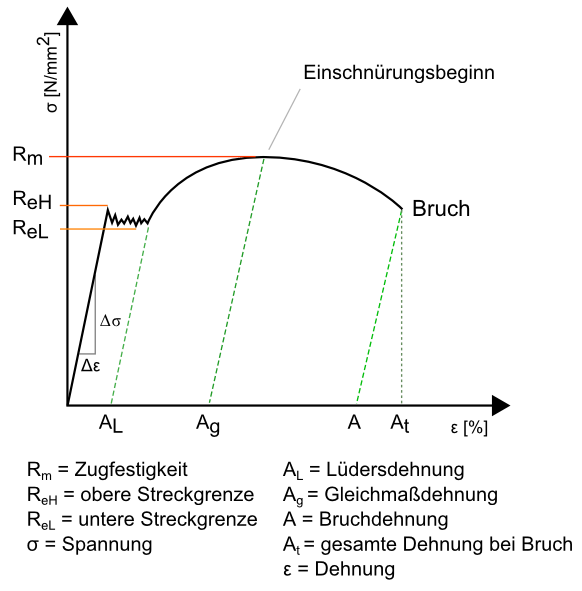
\includegraphics[width=1\linewidth]{img/spannungs-dehnungs-diagramm-06.png}
    \paragraph{Kerbschalgbiegeversuch}
    Kerbschlafarbeit wird oft im Zusammenhang mit der Temepratur gemesse. Wie verhlaten sich Bauteile bi hohen bzw. niedriger temperatur? Duktil oder Spröde?\\
    \begin{minipage}[t]{0.45\columnwidth}
        \begin{itemize}[label={}, leftmargin=*]
            \item \emph{hohe Kerbschlagarbeit:} \\ $\rightarrow$ hohe Duktilität
        \end{itemize}
    \end{minipage}\hfill
    \begin{minipage}[t]{0.55\columnwidth}
        \begin{itemize}[label={}, leftmargin=*]
            \item \emph{tiefe Kerbschlagarbeit:} \\ $\rightarrow$ hohe Sprödigkeit
        \end{itemize}
    \end{minipage}\hfill
    \subsection{Zerstörungsfreie Werkstoffprüfung}
    \paragraph{Sichtprüfung}
    Bauteil immer zuerst Sichten, d.h. Anschauen und in die Hand nehmen. Dabei können potenzielle Fehler schon eingegrenz werden oder ermittelt werden um welches Material es sich handelt.
    \paragraph{Durchstrahlungsprüfung}
    Schwächung der Röntgenstrahlung entsprechend den Dicken- und Dichteverhältnissen
    bei der Durchdringung des Prüfobjektes. \emph{Nachteil}: aufwändige Apparatur, Strahlenschutz notwendig
    \paragraph{Ultraschallprüfung}
    \paragraph{Wirbelstromprüfung}
    \paragraph{Magnetpulverprüfung}
    Alle Arten von Stählen ausser austenit. Entdeckt Fehler die gegen die Feldlinien laufen. Entdeckt nur Fehler an der Oberfläche. Von verschiedenen Seiten Prüfen, dammit alle Fehler sichtbar werden
    \paragraph{Farbeindringprüfung PT(Penetrant Test)}
    Farbeindringmittel wird aufgetragen um Risse an der Oberfläche zu entdecken:\\
    \begin{minipage}[t]{0.70\columnwidth}
        \begin{itemize}[label={}, leftmargin=*, itemsep=0.01em]
            \item \textbf{Vorgehen}:
            \item (Vor-) Reinigen und Trocknen
            \item Eindringvorgang
            \item (Zwischen-) Reinigen und Trocknen
            \item Entwicklungsvorgang und Inspektion
        \end{itemize}
    \end{minipage}\hfill
    \begin{minipage}[t]{0.30\columnwidth}
        \begin{itemize}[label={}, leftmargin=*, itemsep=0.01em]
            \item  \textbf{Eindringmittel} \\ Mineralöl, mit Farbstoffe und
            grenzflächenaktive Additive
            
        \end{itemize}
    \end{minipage}\hfill
    \begin{itemize}[label={}, leftmargin=*, itemsep=0.01em]
        \item \textbf{Zwischenreiniger}: Wasser, lösungsmittel, Emulgatoren
        \item \textbf{Entwickler}: trockenentwickler, feuchtentwickler
    \end{itemize}
    \paragraph{Replika-Methode}
    \subsection{Mechanische Eigenschaften}
    Definition Härte: Widerstand eines Stoffes gegen plastische Formänderung durch das
    Eindringen eines anderen Körpers
    Steifigkeit 
    Festigkeit
    \section*{Aufau von Metallen}
    \paragraph{Gittertypen}\mbox{}\\
    \begin{minipage}[t]{0.32\columnwidth}
        \begin{itemize}[label={}, leftmargin=*,  itemsep=0.01em]
            \item \textbf{kfz}
            \item
            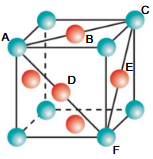
\includegraphics[height=0.5\linewidth]{img/kfz.png}
            \item GE: 6 \\ GR: 2 \\ GS: 12
        \end{itemize}
    \end{minipage}\hfill
    \begin{minipage}[t]{0.32\columnwidth}
        \begin{itemize}[label={}, leftmargin=*,  itemsep=0.01em]
            \item \textbf{krz}
            \item
            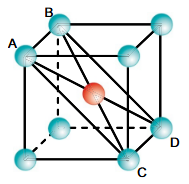
\includegraphics[height=0.5\linewidth]{img/krz.png}
            \item GE: 4 \\ GR: 3 \\ GS: 12
        \end{itemize}
    \end{minipage}\hfill
    \begin{minipage}[t]{0.32\columnwidth}
        \begin{itemize}[label={}, leftmargin=*,  itemsep=0.01em]
            \item \textbf{hdp}
            \item
            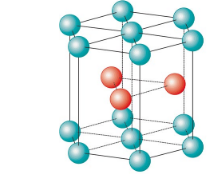
\includegraphics[height=0.5\linewidth]{img/hdp.png}
            \item GE: 1 \\ GR: 3 \\ GS: 3
        \end{itemize}
    \end{minipage}\hfill
    \paragraph{Allotropie}Gitttertyp ändert bei bestmimmten. Temparaturen, bsp Eisen:
    %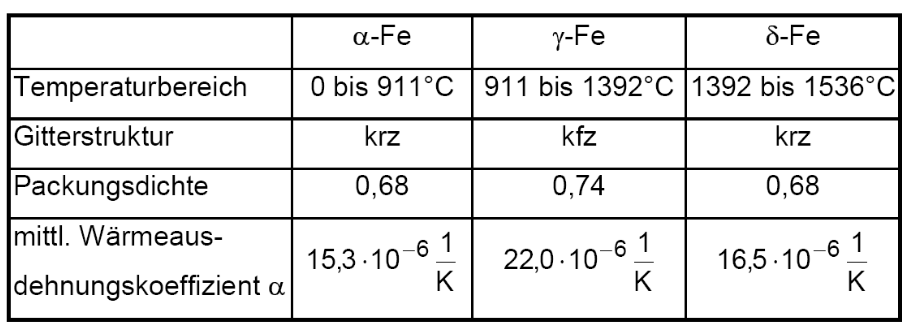
\includegraphics[width=\linewidth]{img/allotropie_eisen.png}
    \paragraph{Phase} Bereich konstanter Struktur und chemischer
    Zusammensetzung.
    \subsection*{Gitterfehler}
     \begin{minipage}[t]{0.5\columnwidth}
        \begin{itemize}[label={}, leftmargin=*, itemsep=0.01em]
            \item \textbf{Nulldimensional (Punktfehler)}
            \item L = Leerstelle \\ S = Substitution \\  ZG = Zwischengitteratom
        \end{itemize}
    \end{minipage}\hfill
    \begin{minipage}[t]{0.5\columnwidth}
        \begin{itemize}[label={}, leftmargin=*,  itemsep=0.01em]
            \item \textbf{Eindimensional (Linienfehler)}
            \item Versetzung = eingeschobene Halbebene
        \end{itemize}
    \end{minipage}\hfill
    \begin{minipage}[t]{0.5\columnwidth}
        \begin{itemize}[label={}, leftmargin=*, itemsep=0.01em]
            \item \textbf{Zweidimensional (Flächenfehler)}
            \item Zwillingsgrenze \\ Stapelfehler \\ Kleinwinkelkorngrenze \\ Grosswinkelkorngrenze
        \end{itemize}
    \end{minipage}\hfill
    \begin{minipage}[t]{0.5\columnwidth}
        \begin{itemize}[label={}, leftmargin=*,  itemsep=0.01em]
            \item \textbf{Dreidimensional (räumliche Fehler)}
            \item Poren \\ Lunker \\ Risse \\ Eischlüsse \\ Auscheidungen 
        \end{itemize}
    \end{minipage}\hfill
    \section*{Legierungen}
    \paragraph{Vollständige Lösbarkeit (Mischkristall)}\mbox{}
    \begin{itemize}[label={}, leftmargin=*,  itemsep=0.01em]
        \item gleicher Gittertyp
        \item Ähnlicher Atomradius ($\Delta < 15\%$)
        \item Ähnliche chemische Eigenschaften
        \item Linsendiagramm "Zigarrendiagramm"
    \end{itemize}
    \paragraph{Vollständige Unlösbarkeit (Kristallgemischlegierung)}\mbox{}
    \begin{itemize}[label={}, leftmargin=*,  itemsep=0.01em]
        \item Umwandlungstemperaturen für alle Zusammensetzungen gleich
        \item Schichtung der flüssigen Komponenten (das leichtere Metall schwimmt auf dem
        schwereren)
        \item Ähnliche chmische Eigenschaften
    \end{itemize}
    \paragraph{Teilweise Lösbarkeit (Gemisch aus Mischkristall)}\mbox{}\\
    In der Praxis treten meisten "Teilweise Lösbarkeit" auf als Substitutionsmischkirstalle oder Einlagerungsmischkristalle.
    \begin{itemize}[label={}, leftmargin=*, itemsep=0.01em]
        \item $\alpha$-Kistall: Hauptanteil Grundelement Substitution oder Einlagerung durch Legierungselement
        \item $\beta$-Kistall: Hauptanteil Legierungselement Substitution oder Einlagerung durch Grundelement
    \end{itemize}
    \section{Werkstoffklasse Metalle}
    \paragraph{Eisen}\mbox{}\\
        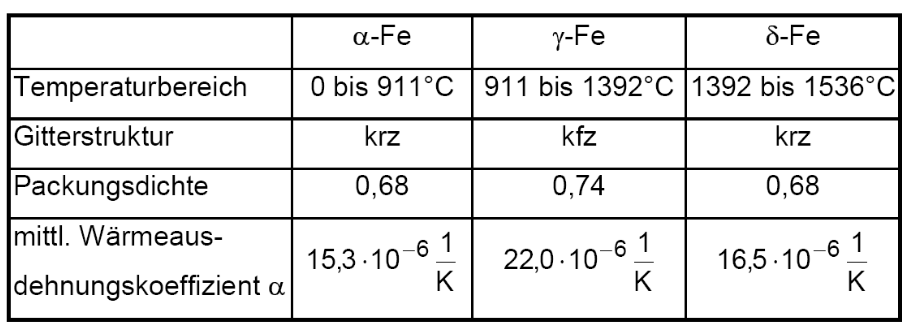
\includegraphics[width=0.8\linewidth]{img/allotropie_eisen.png}
        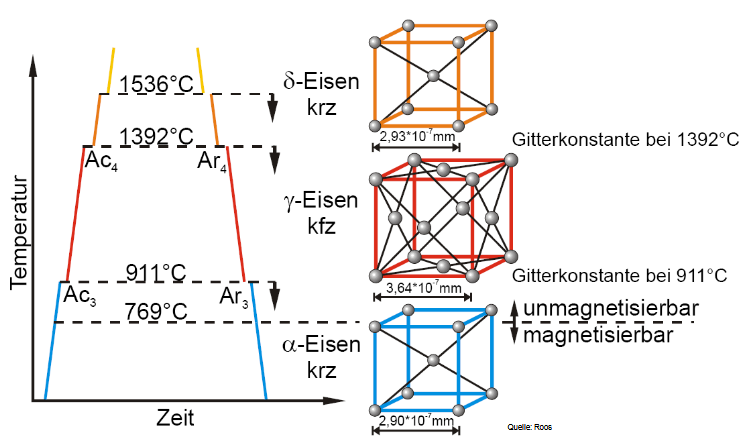
\includegraphics[height=0.5\linewidth]{img/allotropie_eisen_grafik.png}
    \paragraph{Stahl}
    Fe-C-Legierung: C < 2\% und Mn < 1\%
    \paragraph{Einteilung nach Verwendungszweck}
    \begin{minipage}[t]{0.5\columnwidth}
        \begin{itemize}[label={}, leftmargin=*, itemsep=0.01em]
            \item \textbf{Baustähle}
            \item Basiswerkstoffe für den Konstrukteur (Maschinen, Anlagen,
            Fahrzeuge etc.)
        \end{itemize}
    \end{minipage}\hfill
    \begin{minipage}[t]{0.5\columnwidth}
        \begin{itemize}[label={}, leftmargin=*,  itemsep=0.01em]
            \item \textbf{Werkzeugstähle}
            \item Werkzeuge für die Formgebung (Umformen, Giessen, Spanen)
        \end{itemize}
    \end{minipage}
    \begin{minipage}[t]{0.5\columnwidth}
        \begin{itemize}[label={}, leftmargin=*, itemsep=0.01em]
            \item \textbf{warmfeste Stähle}
            \item Einsatz bei hoher Temperatur (Energietechnik, Kraftwerke)
        \end{itemize}
    \end{minipage}\hfill
    \begin{minipage}[t]{0.5\columnwidth}
        \begin{itemize}[label={}, leftmargin=*,  itemsep=0.01em]
            \item \textbf{rostbeständige Stähle}
            \item Chromgehalt > 12\% $\rightarrow$ Chromoxidschicht
        \end{itemize} 
    \end{minipage}\hfill
    \paragraph{Einteilung nach metallphysikalischen Merkmalen }
    \begin{minipage}[t]{0.5\columnwidth}
        \begin{itemize}[label={}, leftmargin=*, itemsep=0.01em]
            \item \textbf{ferritsche Stähle}
            \item $\alpha$-Mk \\ krz \\ ausgeprägte Sreckgrenze \\ spröd bei tiefen Temp.
        \end{itemize}
    \end{minipage}\hfill
    \begin{minipage}[t]{0.5\columnwidth}
        \begin{itemize}[label={}, leftmargin=*,  itemsep=0.01em]
            \item \textbf{Perlitische}
            \item $\alpha$-Mk \\ krz \\ eutektoide Umwandlung bei 0.8 \% C.
        \end{itemize}
    \end{minipage}
    \begin{minipage}[t]{0.5\columnwidth}
        \begin{itemize}[label={}, leftmargin=*, itemsep=0.01em]
            \item \textbf{Austenit}
            \item $\gamma$-Mk \\ kfz \\ sehr duktil \\ gute kalt-Formabrakeit
        \end{itemize}
    \end{minipage}\hfill
    \begin{minipage}[t]{0.5\columnwidth}
        \begin{itemize}[label={}, leftmargin=*,  itemsep=0.01em]
            \item \textbf{Martensit}
            \item $\alpha$-Mk verzerrt \\ kfz \\ C > 0.2\% \\ gehärtetes Gefüge
        \end{itemize} 
    \end{minipage}\hfill
    \paragraph{Eisen-Kohlenstoff-Diagramm}
    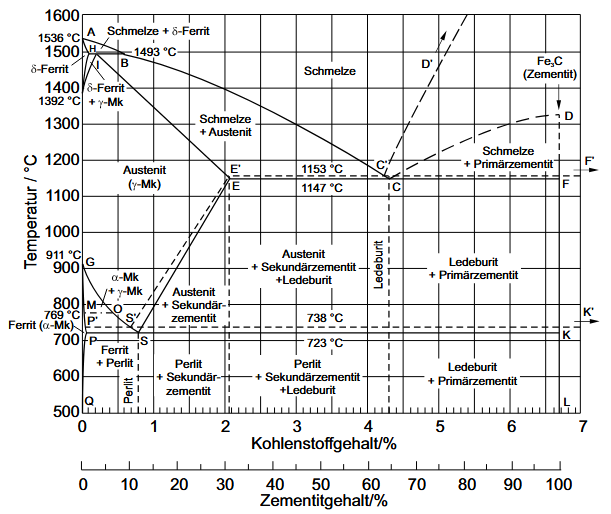
\includegraphics[width=\linewidth]{img/eisen_kohlenstoff_diagramm.png}
    \paragraph{DIN EN 10027-1}
    \paragraph{Aluminum}\mbox{}\\
    \begin{minipage}[t]{0.5\columnwidth}
        \begin{itemize}[label={}, leftmargin=*, itemsep=0.01em]
            \item \textbf{Eigenschaften}
            \item Dichte 2.7 $\frac{g}{m^3}$\\ Schmelztemperatur: 666°C \\ Gitter: kfz \\ E-Modul: 70GPa \\ Korrosionsbeständigkeit ($Al_2O_3$-Deckschicht)
        \end{itemize}
    \end{minipage}\hfill
    \begin{minipage}[t]{0.5\columnwidth}
        \begin{itemize}[label={}, leftmargin=*,  itemsep=0.01em]
            \item \textbf{Einteilung}
            \item \textbf{Reinalluminium} \\ \textbf{Legierung}: aushärtbat \& nicht aushärtbar $\rightarrow$ \textbf{Knetlegierung} \& Gusslegierung \\ Aluminium-Sinter
        \end{itemize} 
    \end{minipage}\hfill
    \paragraph{Kennzeichnung-Aluminium}\mbox{}\\
    TBD Folie 21-24 in Vorlseung\\
    \begin{minipage}[t]{0.35\columnwidth}
        \begin{itemize}[label={}, leftmargin=*,  itemsep=0.01em]
            \item \textbf{Gussverfahren}
            \item Druckguss \\ Kokillenguss \\ Sandguss
        \end{itemize}
    \end{minipage}\hfill
    \begin{minipage}[t]{0.65\columnwidth}
        \begin{itemize}[label={}, leftmargin=*,  itemsep=0.01em]
            \item \textbf{Gusslegierung}
            \item hoch legiert (Si \& Mn) \\ eutektisch (nahe 12\% Si) \\ geringe Löslichkeit von Si in Al
        \end{itemize}
    \end{minipage}\hfill
    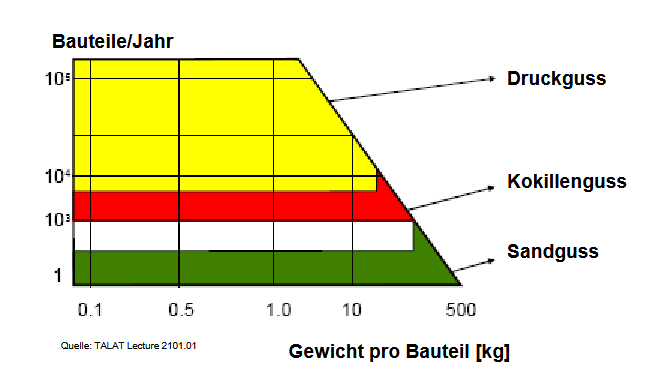
\includegraphics[height=0.5\linewidth]{img/gussverfahren_aluminium.png}
    \begin{minipage}[t]{0.32\columnwidth}
        \begin{itemize}[label={}, leftmargin=*,  itemsep=0.01em]
            \item \textbf{Druckguss}
        \end{itemize}
    \end{minipage}\hfill
    \begin{minipage}[t]{0.32\columnwidth}
        \begin{itemize}[label={}, leftmargin=*,  itemsep=0.01em]
            \item \textbf{Kokillengusss}
        \end{itemize}
    \end{minipage}\hfill
    \begin{minipage}[t]{0.32\columnwidth}
        \begin{itemize}[label={}, leftmargin=*,  itemsep=0.01em]
            \item \textbf{Sandguss}
        \end{itemize} 
    \end{minipage}\hfill
    \begin{minipage}[t]{\columnwidth}
        \begin{itemize}[label={}, leftmargin=*,  itemsep=0.01em]
            \item \textbf{Alluminum-Gusslegierung} \\ Aluminiumgusslegierungen enthalten höhere Gehalte an
            Legierungselementen als Knetlegierungen: vor allem Si und Mg \\ eutektische Legierungssysteme (nahe 12\% Si) \\ geringe Löslichkeit von Si in Al
        \end{itemize} 
    \end{minipage}\hfill
    \subsection{Titan}
    \begin{minipage}[t]{0.5\columnwidth}
        \begin{itemize}[label={}, leftmargin=*, itemsep=0.01em]
            \item \textbf{Eigenschaften}
            \item Dichte 4.5 $\frac{g}{m^3}$\\ Schmelztemperatur: 1668°C \\ hdp $\alpha$-TI, krz $\beta$-TI (Grenzee 882°C) \\ E-Modul: 115GPa \\ Korrosionsbeständigkeit ($TiO_2$-Deckschicht)
        \end{itemize}
    \end{minipage}\hfill
    \begin{minipage}[t]{0.5\columnwidth}
        \begin{itemize}[label={}, leftmargin=*,  itemsep=0.01em]
            \item \textbf{Legierungen}
            \item \textbf{neutral} Sn,Zr \\ \textbf{$\alpha$-stabiliserend} Ai,O,N,C \\ \textbf{$\beta$-isomorph} MO,V,Ta,Nb \\ \textbf{$\beta$-eutektiode} FE,Mn,Cr,Co,Ni,Cu,Si,H
        \end{itemize} 
    \end{minipage}\hfill
    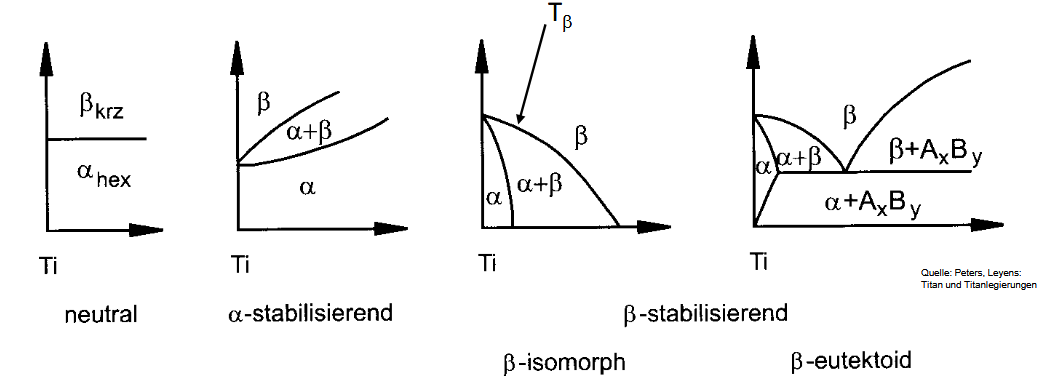
\includegraphics[width=\linewidth]{img/titan_legierungen.png}
    \paragraph{Klassifizierung von Titan}
    \begin{minipage}[t]{\columnwidth}
        \begin{itemize}[label={}, leftmargin=*,  itemsep=0.01em]
            \item $\alpha$: ausschliesslich $\alpha$-stabilisierende Elemente \\ near-$\alpha$: geringe Anteile an $\beta$-stabilisierenden Elementen \\ $\alpha+\beta$ zweiphasig, bimodal \\ metastabil-$\beta$: hoher Anteil an $\beta$-stabilisierenden Elementen, zweiphasig \\ $\beta$: einphasig
        \end{itemize} 
    \end{minipage}\hfill
    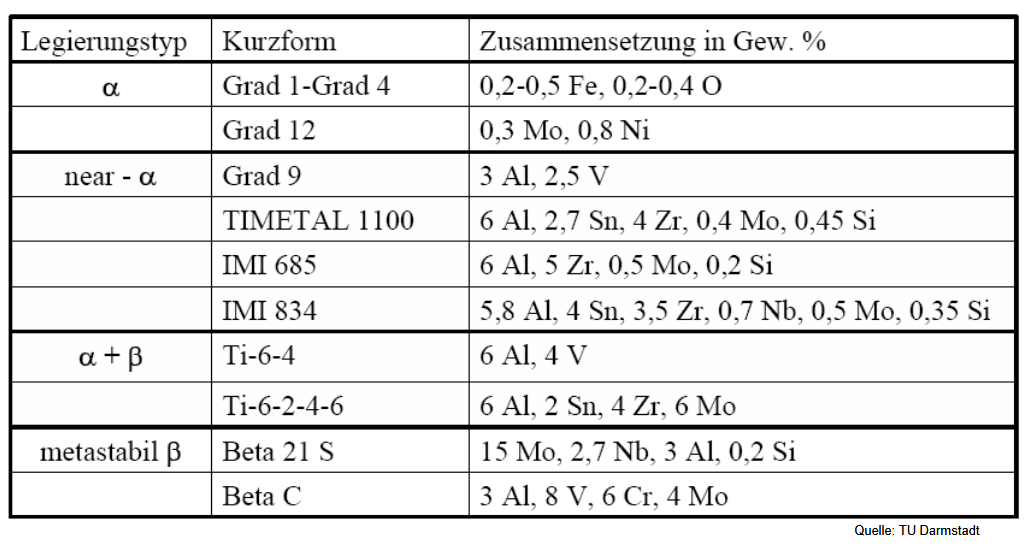
\includegraphics[width=\linewidth]{img/klassifizierung_titan.png}
    \paragraph{Eigenschaften von Titan}
    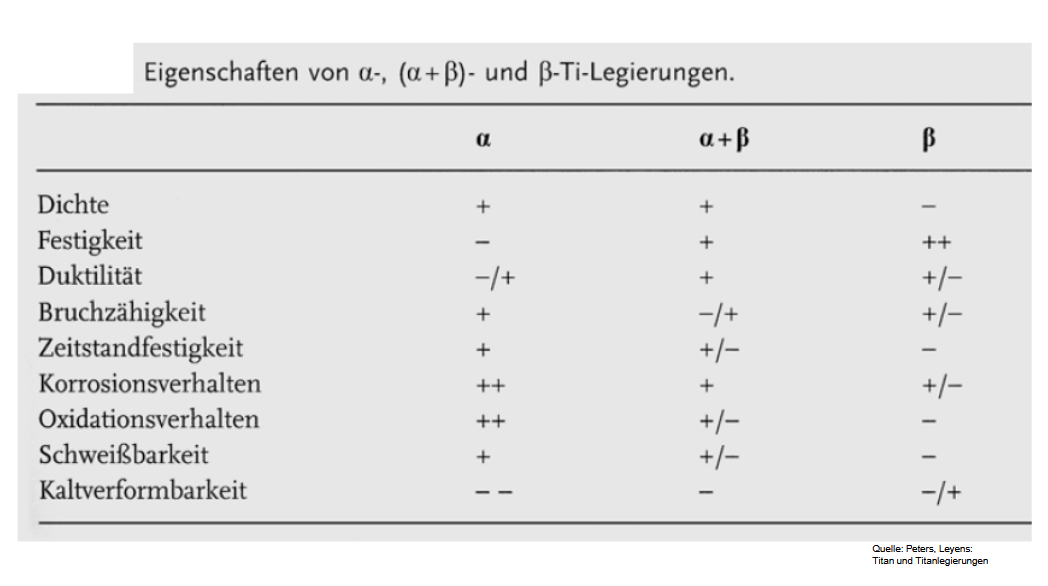
\includegraphics[width=\linewidth]{img/eigenschaften_von_titan.png}
    \paragraph{Anwendungen von Titan}\mbox{}\\
    \begin{minipage}[t]{0.5\columnwidth}
        \begin{itemize}[label={}, leftmargin=*, itemsep=0.01em]
            \item \textbf{$\alpha$-Titan} \\ Dentalbereich \\ Knochenplatten- schrauben \\ Pfannenbeschichtungen \\ formbare Implantate
        \end{itemize}
    \end{minipage}\hfill
    \begin{minipage}[t]{0.5\columnwidth}
        \begin{itemize}[label={}, leftmargin=*, itemsep=0.01em]
            \item \textbf{Metastabile-$\beta$-Titan} \\ aushärtbar \\ Streckgrenzen bis über 1400 MPa möglich \\ krz Matrix \\ Umformung bei Raumtemperatur möglich \\ Luftfahrt
        \end{itemize}
    \end{minipage}\hfill
    \begin{minipage}[t]{1\columnwidth}
        \begin{itemize}[label={}, leftmargin=*,  itemsep=0.01em]
            \item \textbf{$\alpha+\beta$-Titan} \\ \textbf{gebräuchlichste Titanlegierungen} $\rightarrow$ „Klassiker“: Ti6Al4V (= Ti Grade 5), ca. 50 \% der Weltproduktion \\ \textbf{hohe Festigkeit} ($R_{p0,2}$ $\approx$ 1000 MPa) \\ \textbf{hohe Bruchzähigkeit} (60 – 110 MPa m 1/2 ) \\ am meisten erforschte und erprobte Legierungsklasse \\ Wirbelsäuleschrauben \\ Bandscheibe
        \end{itemize} 
    \end{minipage}\hfill
    \subsection{Magnesium}
    \begin{minipage}[t]{0.5\columnwidth}
        \begin{itemize}[label={}, leftmargin=*, itemsep=0.01em]
            \item \textbf{Eigenschaften}
            \item Dichte 1.74 $\frac{g}{m^3}$\\ Schmelztemperatur: 650°C \\ Gittertyp: hdp \\ E-Modul: 45GPa \\ geringe Korrosionsbeständigkeit \\ exellente giessbarkeit
        \end{itemize}
    \end{minipage}\hfill
    \begin{minipage}[t]{0.5\columnwidth}
        \begin{itemize}[label={}, leftmargin=*,  itemsep=0.01em]
            \item \textbf{tbd}
            \item
        \end{itemize} 
    \end{minipage}\hfill
    \paragraph{Kennzeichnung Magnesium}
    \paragraph{Verarbeitung von Magnesium}\mbox{}\\
    \begin{minipage}[t]{0.5\columnwidth}
        \begin{itemize}[label={}, leftmargin=*, itemsep=0.01em]
            \item \textbf{Gusslegierung}
            \item div. Gussaurteb \\ 90\% aller Bauteile Guss \\ Autoindustrie und Gehäuse
        \end{itemize}
    \end{minipage}\hfill
    \begin{minipage}[t]{0.5\columnwidth}
        \begin{itemize}[label={}, leftmargin=*,  itemsep=0.01em]
            \item \textbf{Kentlegierung}
            \item Gitter: hdp $\rightarrow$ schlecht Kaltformbar \\  gute Warmumformbarkeit \\ Halbzeuge (Rohre, Bleche, Profile, etc.) \\ Felgen \& Gehäuse \\ Med. Stent
        \end{itemize} 
    \end{minipage}\hfill
    \subsection{Kupfer}
    \begin{minipage}[t]{0.5\columnwidth}
        \begin{itemize}[label={}, leftmargin=*, itemsep=0.01em]
            \item \textbf{Eigenschaften}
            \item Dichte 8.93 $\frac{g}{m^3}$\\ Schmelztemperatur: 1083°C \\ Gittertyp: kfz \\ E-Modul: 45GPa \\  Korrosionsbeständigkeit ($Cu_20$)\\ gut Umformbarkeit
        \end{itemize}
    \end{minipage}\hfill
    \begin{minipage}[t]{0.5\columnwidth}
        \begin{itemize}[label={}, leftmargin=*,  itemsep=0.01em]
            \item \textbf{Bezeichnung von Kupfer} 
            \item Messing $\rightarrow$ CuZn10 : Cu mit 10 Gew.-\% Zink (Zn) \\ Bronze $\rightarrow$ CuSn6: Cu mit 6 Gew.-\% Zinn (Sn) \\ Rotguss $\rightarrow$ CuSn5Zn5Pb5-C: Cu mit 5 Gew.-\% Sn + 5 Gew.-\% Zn + 5 Gew.-\% Pb
        \end{itemize} 
    \end{minipage}\hfill
    \subsection{Smart Materials Formgedächtnislegierungen}
    \begin{minipage}[t]{0.32\columnwidth}
        \begin{itemize}[label={}, leftmargin=*, itemsep=0.01em]
            \item \textbf{Einweg-Effekt}
            \item Belasten bei Raumtemperatur \\ Bauteilverformt isch bleibend \\ Wärmebehandlung $T > A_f$ \\Bauteil nimmt ursprüngliche gestalt an.
        \end{itemize}
    \end{minipage}\hfill
    \begin{minipage}[t]{0.32\columnwidth}
        \begin{itemize}[label={}, leftmargin=*,  itemsep=0.01em]
            \item \textbf{Zweiweg-Effekt} 
            \item Erwäremen \\ Bauteil verformt sich \\ Abkühlen \\ Bauteil nimmt ursprüngliche Form an
        \end{itemize} 
    \end{minipage}\hfill
    \begin{minipage}[t]{0.32\columnwidth}
        \begin{itemize}[label={}, leftmargin=*,  itemsep=0.01em]
            \item \textbf{Pseudoelsatzität} 
            \item Belasten bei Raumtemepratur \\ Bauteil verformt sich \\ Entlasten \\ Bauteil nimmt ursprüngliche Form an
        \end{itemize} 
    \end{minipage}\hfill
    \section{Wärmebehandlung}\mbox{}\\
    \begin{minipage}[t]{1\columnwidth}
        \begin{itemize}[label={}, leftmargin=*,  itemsep=0.01em]
            \item \textbf{Zweck der Wärmebehandlung} 
            \item Herabsetzung/Steigerung von Härte/Festigkeit \\ Verbesserung von Zähigkeit und Umformbarkeit \\ Verbesserung von Zähigkeit und Umformbarkeit \\ Verbesserung von Zähigkeit und Umformbarkeit \\ Abbau von Eigenspannungen
        \end{itemize} 
    \end{minipage}\hfill
    \begin{minipage}[t]{0.5\columnwidth}
        \begin{itemize}[label={}, leftmargin=*,  itemsep=0.01em]
            \item \textbf{Weichglühen} 
            \item Vermindern der Härte, Verbessern der Zerspanbarkeit \\ Stahl: $T < A_1 (723°C)$ mit langsamen Abkühle
        \end{itemize} 
    \end{minipage}\hfill
    \begin{minipage}[t]{0.5\columnwidth}
        \begin{itemize}[label={}, leftmargin=*,  itemsep=0.01em]
            \item \textbf{Spannungsarmglüühen} 
            \item nach dem Schweissen \\ Glühung bei 550°C...650°C mit langsamem Abkühlen \\ 
        \end{itemize} 
    \end{minipage}\hfill
    \begin{minipage}[t]{1\columnwidth}
        \begin{itemize}[label={}, leftmargin=*,  itemsep=0.01em]
            \item \textbf{statische Rekristallisation} 
            \item hebt die Kaltverfestigung auf und reduziert die Fliessspannung \\ Umformgrade = mehrfaches Rekristallisationsglühungen \\ Keimbildung neuer, versetzungsarmer Körner \\ Wachstum auf Kosten der Nachbarkörner (hohe Versetzungsdichte) \\ Entstehung eines neuen Gefüges \\ $T_{rekr} \approx 0.4T_s$
        \end{itemize}
    \end{minipage}
    \begin{minipage}[t]{1\columnwidth}
        \begin{itemize}[label={}, leftmargin=*,  itemsep=0.01em]
            \item \textbf{dynamische Rekristallisation} 
            \item gleichzeitiges Umformen und Rekrsitallisieren
        \end{itemize}
    \end{minipage}\hfill
    \begin{minipage}[t]{1\columnwidth}
        \begin{itemize}[label={}, leftmargin=*,  itemsep=0.01em]
            \item \textbf{Auscheidungshärten} 
            \item Widerstand für Versetzungsbewegung \\ Festigkeit (v.a. Streckgrenze) $\uparrow$ \\ Raumtemperatur: Kaltauslagern \\ $T \le 200°C$: Warmauslagern
        \end{itemize}
    \end{minipage}\hfill
    \begin{minipage}[t]{1\columnwidth}
        \begin{itemize}[label={}, leftmargin=*,  itemsep=0.01em]
            \item \textbf{ZTU-Diagramm} 
            \item isotherm: schnelle abkühlung $\rightarrow$ ideal \\ kontinureilich: stetige abkühlung $\rightarrow$ real
        \end{itemize}
    \end{minipage}\hfill
    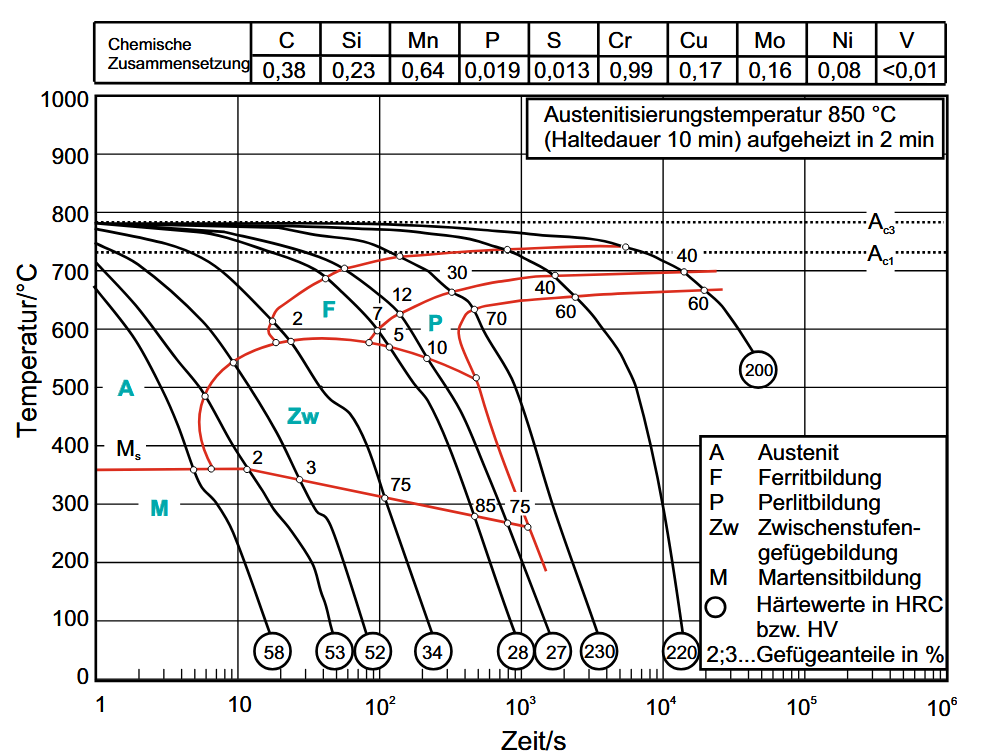
\includegraphics[width=\linewidth]{img/ztu_diagramm.png}
    \begin{minipage}[t]{1\columnwidth}
        \begin{itemize}[label={}, leftmargin=*,  itemsep=0.01em]
            \item \textbf{Stahl härten} 
            \item Ziel: harte, verschleissbeständige Oberfläche \\ Erhöhung der statischen und dynamischen Festigkeit
            \item Voraussetzung : Mindestkohlenstoffgehalt von 0,2..0,3\% bei unlegierten
            Stählen
            \item Abfolge: Austenitisieren \\ abschrecken
        \end{itemize}
    \end{minipage}\hfill
    \paragraph{Härtemethoden}\mbox{}\\
    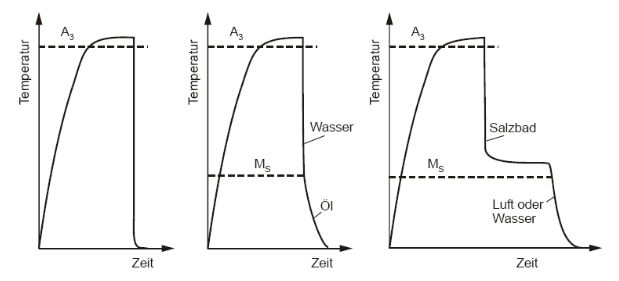
\includegraphics[width=\linewidth]{img/härte_methoden.png}
    \paragraph{Abkühlmedium}\mbox{}\\
    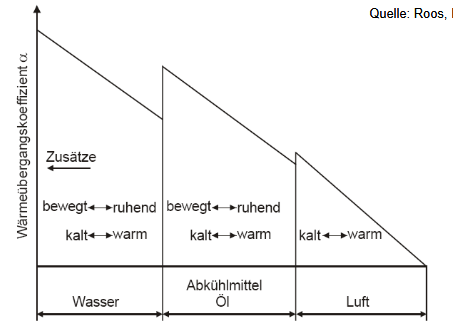
\includegraphics[width=\linewidth]{img/abkühlmedium.png}
    \begin{minipage}[t]{1\columnwidth}
        \begin{itemize}[label={}, leftmargin=*,  itemsep=0.01em]
            \item \textbf{Induktionshärten} 
            \item Erhitzen Reanbereich mit Induktion \\ Abschrecken im Wasser
        \end{itemize}
    \end{minipage}\hfill
    \begin{minipage}[t]{1\columnwidth}
        \begin{itemize}[label={}, leftmargin=*,  itemsep=0.01em]
            \item \textbf{Flammenhärten und Laserhärten} 
            \item Erhitzen de Oberfläche mit Laser oder Flamme
        \end{itemize}
    \end{minipage}\hfill
    \begin{minipage}[t]{1\columnwidth}
        \begin{itemize}[label={}, leftmargin=*,  itemsep=0.01em]
            \item \textbf{Einsatzhärten} 
            \item kohlenstoffarme, unlegierte Stähle bzw. legierte Stähle mit C < 0,2\% \\ Eindiffusion von Kohlenstoff (C) oberhalb A 3 (= Aufkohlen
        \end{itemize}
    \end{minipage}\hfill
    \section{Polymere}
    \paragraph{Synthese von Kunststoffen}\mbox{}\\
    \begin{minipage}[t]{0.32\columnwidth}
        \begin{itemize}[label={}, leftmargin=*, itemsep=0.01em]
            \item \textbf{P-merisation}
            \item Aufbrechen C=C-Doppelbindung 
            \item Typisch: : PS, PVC, PMMA, PE, POM, PTFE, PP
        \end{itemize}
    \end{minipage}\hfill
    \begin{minipage}[t]{0.32\columnwidth}
        \begin{itemize}[label={}, leftmargin=*,  itemsep=0.01em]
            \item \textbf{P-kondensation}
            \item Verknüpfung gleicher oder verschiedenartiger Moleküle unter
            Abspaltung eines niedermolekularen Stoffes
            \item typisch für PA, PC, PET, PF, UF, UP
        \end{itemize} 
    \end{minipage}\hfill
    \begin{minipage}[t]{0.32\columnwidth}
        \begin{itemize}[label={}, leftmargin=*, itemsep=0.01em]
            \item \textbf{P-addition}
            \item Bildung von Makromolekülen durch Reaktion zweier Partner oder
            Umlagerung von Atomen oder Atomgruppen im Molekül ohne Abspaltung
            von Nebenprodukten
            \item typisch Polyurethan (PUR), EP, POM
        \end{itemize}
    \end{minipage}\hfill
    \paragraph{Typen von Kunststoffen}\mbox{}\\
    \begin{itemize}[label={}, leftmargin=*,  itemsep=0.01em]
        \item gute chemische Beständigkeit (bei Raumtemperatur)
        \item niedrige Dichte $(0.9 g/cm^3 < \rho < 2.2 g/cm^3 )$
        \item niedriger Elastizitätsmodul
        \item geringe Wärmeleitfähigkeit (keine frei beweglichen Elektronen)
        \item hohes Dämpfungsvermögen
        \item geringe elektrische Leitfähigkeit (Isolator, keine frei beweglichen Elektronen)
        \item Sprödigkeit bei niedriger Temperatur und geringe Festigkeit bei hoher
        Temperatur
    \end{itemize}
    \begin{center}
        \small
        \begin{tabular}{|l|c|c|}
            \hline
            \textbf{Eigenschaft} & \textbf{nicht vernetzt} & \textbf{vernetzt} \\
            \hline
            Struktur & linear / verzweigt & 3D-Netz \\
            \hline
            Bindungen & keine Querver. & chem. Querver. \\
            \hline
            Schmelzen & ja & nein \\
            \hline
            Umformen & ja & nein \\
            \hline
            Wärmebest. & gering & hoch \\
            \hline
            Verhalten & plastisch & elast./spröde \\
            \hline
            Typ & Thermoplast & Elastomer / Duroplast \\
            \hline
        \end{tabular}
    \end{center}
    
    
    \section{Fachwörter}
     \begin{minipage}[t]{0.32\columnwidth}
        \begin{itemize}[label={}, leftmargin=*, itemsep=0.01em]
            \item \textbf{stabil}
            \item niedrigste freie Energie \\ bleibt dauerhaft bestehen \\ z. B. Ferrit + Zementit bei Raumtemperatur
        \end{itemize}
    \end{minipage}\hfill
    \begin{minipage}[t]{0.32\columnwidth}
        \begin{itemize}[label={}, leftmargin=*,  itemsep=0.01em]
            \item \textbf{metastabil}
            \item nicht energetisch minimal \\ bleibt bestehen wegen kinetischer Barrieren \\ Martensit bei Raumtemperatur
        \end{itemize} 
    \end{minipage}\hfill
    \begin{minipage}[t]{0.32\columnwidth}
        \begin{itemize}[label={}, leftmargin=*, itemsep=0.01em]
            \item \textbf{instabil}
            \item kein lokales Energieminimum \\ wandelt sich spontan und ohne Barriere um \\ $T_{Schemlze} < T_s $
        \end{itemize}
    \end{minipage}\hfill
\end{document}
